\documentclass{beamer}

\mode<presentation> {
  \usetheme{Madrid}
  \setbeamercovered{transparent}
}

\usepackage[czech]{babel}
\usepackage[utf8]{inputenc}
\usepackage{graphicx}
\usepackage{hyperref}

\title{Barevné souřadnice}
\author{Drahomír Dlabaja}
\institute[xdlaba02]{Vysoké učení technické v Brně}
\date{\today}

\begin{document}

\begin{frame}
  \titlepage
\end{frame}

\begin{frame}
  \center
  \frametitle{Gamut prostoru sRGB?}
  \begin{figure}
    \includegraphics[height=0.7\textheight]{CIExy1931_sRGB.png}
  \end{figure}
  To je ten trojúhelník uprostřed té velké věci.
\end{frame}

\begin{frame}
  \center
  \frametitle{Tři senzory lidského oka}
  Každý senzor reaguje na vlnové délky jinak, ale reakce se překrývají.
  \begin{figure}
    \includegraphics[height=0.6\textheight]{Cones_SMJ2_E.pdf}
  \end{figure}
  Co když mozek dostane signál pouze ze senzoru \texttt{M}?
\end{frame}

\begin{frame}
  \center
  \frametitle{Citlivost lidského oka}
  Monochromatické světlo o 620 nm musí mít dvakrát takovou intenzitu oproti 560 nm, aby bylo vnímáno se stejným jasem.
  \begin{figure}
    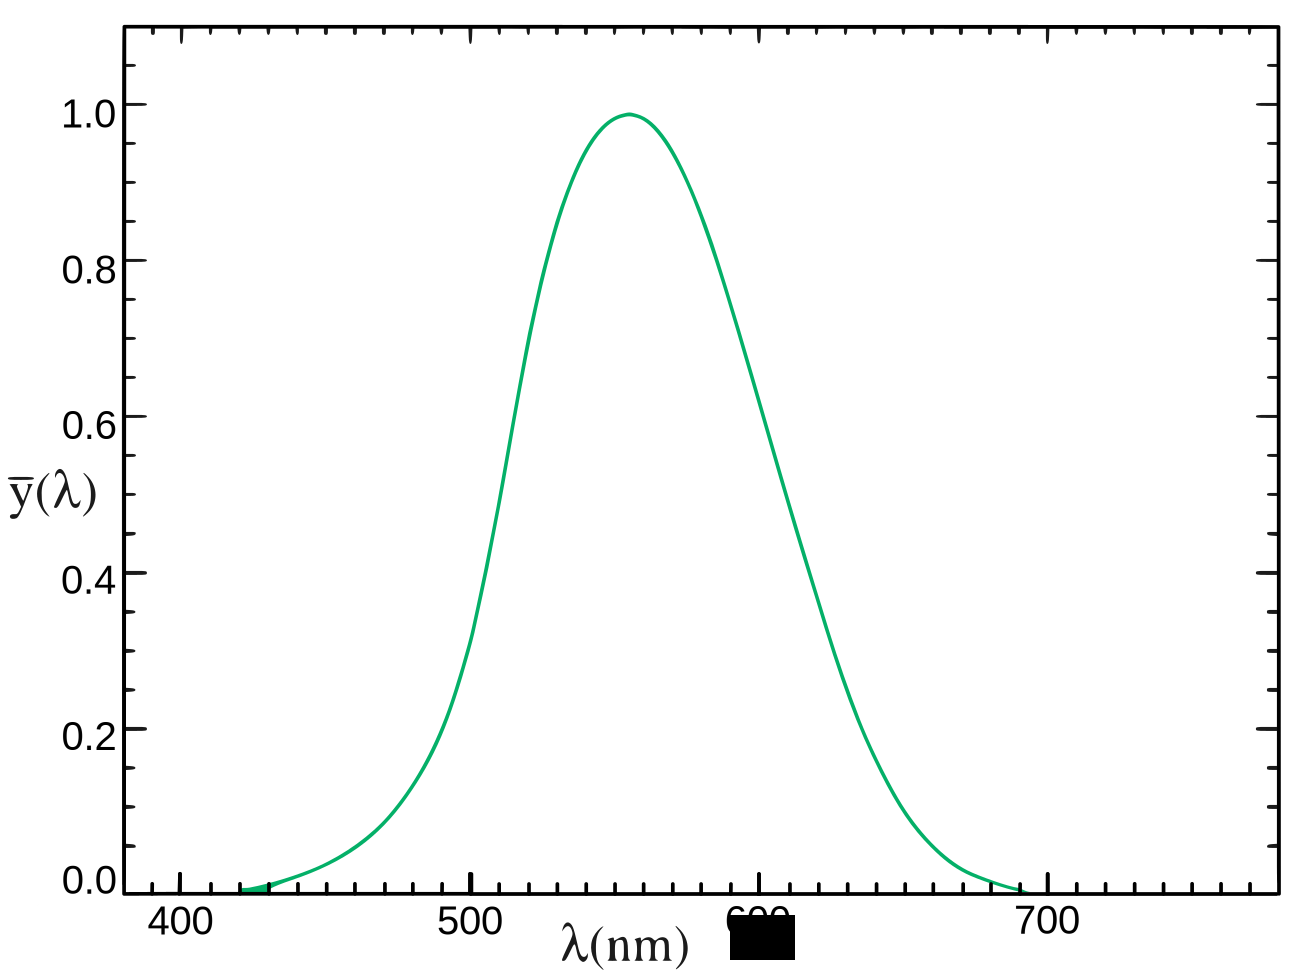
\includegraphics[height=0.6\textheight]{CIE_1931_Luminosity.pdf}
  \end{figure}
\end{frame}

\begin{frame}
  \center
  \frametitle{Experimenty CIE RGB 1931}
  Tři zdroje světla generují spoustu kombinací LMS $\rightarrow$ spoustu barev.
  \begin{figure}
    \includegraphics[height=0.5\textheight]{observer.png}
    \footnote{\url{https://medium.com/hipster-color-science/a-beginners-guide-to-colorimetry-401f1830b65a}}
  \end{figure}
  Nikdy ale ne všechny.
\end{frame}

\begin{frame}
  \center
  \frametitle{CIE RGB 1931}
  Záporné hodnoty $\rightarrow$ vlnové délky nelze pomocí CIE RGB simulovat.
  \begin{figure}
    \includegraphics[height=0.6\textheight]{CIE1931_RGBCMF.pdf}
  \end{figure}
  Leda bychom měli světlo se zápornou intenzitou.
\end{frame}

\begin{frame}
    \center
  \frametitle{CIE RGB $\rightarrow$ CIE rgb}
  Nezajímá nás jas, ale jen chromaticita $\rightarrow$ normalizujeme.

  \begin{align}
    \begin{split}
    r &= R / (R + G + B)\\
    g &= G / (R + G + B)\\
    b &= B / (R + G + B)
  \end{split}
    \label{eq:rgb}
  \end{align}

  \begin{align}
    r+g+b=1
  \end{align}

  Souřadnici \textit{b} nepotřebujeme, protože jde dopočítat.
\end{frame}

\begin{frame}
  \center
  \frametitle{CIE rgb 1931}
  \begin{itemize}
    \item \textbf{Lokus} -- monochromatické barvy.
    \item \textbf{Gamut} -- všechny kombinace monochromatických barev.
    \item \textbf{Ten zbytek} -- imaginární barvy (reaguje např. jenom senzor \texttt{M}).
  \end{itemize}
  \begin{figure}
    \includegraphics[height=0.6\textheight]{CIE1931_rgxy.png}
  \end{figure}
  Bylo by fajn, kdybychom nemuseli pracovat se zápornými souřadnicemi.
\end{frame}

\begin{frame}
  \center
  \frametitle{Lineární transforamce CIE rgb 1931 $\rightarrow$ CIE xyz 1931}
  Základní barvy jsou teď imaginární, ale to ničemu nevadí.
  \begin{figure}
    \includegraphics[height=0.6\textheight]{CIE1931xy_CIERGB.pdf}
  \end{figure}
  Máme objektivní model lidského vidění barev.
\end{frame}

\begin{frame}
  \center
  \frametitle{Denormalizace CIE xyz $\rightarrow$ CIE XYZ}
  Barvy v grafu jsou spíše matoucí, s RGB už to nemá moc společného.
  \begin{figure}
    \includegraphics[height=0.6\textheight]{CIE_1931_XYZ_Color_Matching_Functions.pdf}
  \end{figure}
  Křivka \texttt{Y} odpovídá funkci citlivosti lidského oka $\rightarrow$ z barvy hned známe jas.\\
  Což je praktické.
\end{frame}

\begin{frame}
  \frametitle{Co je teda ten gamut prostoru sRGB}
  \center
\begin{minipage}{0.6\linewidth}
  \begin{itemize}
    \item Základní barvy už nejsou na loku(su?) $\rightarrow$ to nevadí, monochromatické zdroje jsou drahé anyway. Hlavně že jsou reálné.
    \item Uvnitř trojúhelníku jsou všechny barvy vyjádřitelné v sRGB.
    \item Spousta barev nevyjádřitelných $\rightarrow$ máme i prostory s větším gamutem (Adobe RGB).
    \item D65 jsou souřadnice bílé barvy. Existuje spousta bílých barev, ale o tom jindy.
  \end{itemize}
\end{minipage}%
\begin{minipage}{0.4\linewidth}
  \begin{figure}
    \center
    \includegraphics[width=\linewidth]{CIExy1931_sRGB.png}
  \end{figure}
\end{minipage}\\[2em]
Dosud jsme ignorovali třetí dimezi $\rightarrow$ vizte vizualizační appku.
\end{frame}


\end{document}
